\documentclass[11pt]{article}
\usepackage{geometry,marginnote} % Pour passer au format A4
\geometry{hmargin=1cm, vmargin=1cm} % 

% Page et encodage
\usepackage[T1]{fontenc} % Use 8-bit encoding that has 256 glyphs
\usepackage[english,french]{babel} % Français et anglais
\usepackage[utf8]{inputenc} 

\usepackage{lmodern,numprint}
\setlength\parindent{0pt}

% Graphiques
\usepackage{graphicx,float,grffile,units}
\usepackage{tikz,pst-eucl,pst-plot,pstricks,pst-node,pstricks-add,pst-fun,pgfplots} 

% Maths et divers
\usepackage{amsmath,amsfonts,amssymb,amsthm,verbatim}
\usepackage{multicol,enumitem,url,eurosym,gensymb,tabularx}

\DeclareUnicodeCharacter{20AC}{\euro}



% Sections
\usepackage{sectsty} % Allows customizing section commands
\allsectionsfont{\centering \normalfont\scshape}

% Tête et pied de page
\usepackage{fancyhdr} \pagestyle{fancyplain} \fancyhead{} \fancyfoot{}

\renewcommand{\headrulewidth}{0pt} % Remove header underlines
\renewcommand{\footrulewidth}{0pt} % Remove footer underlines

\newcommand{\horrule}[1]{\rule{\linewidth}{#1}} % Create horizontal rule command with 1 argument of height

\newcommand{\Pointilles}[1][3]{%
  \multido{}{#1}{\makebox[\linewidth]{\dotfill}\\[\parskip]
}}

\newtheorem{Definition}{Définition}

\usepackage{siunitx}
\sisetup{
    detect-all,
    output-decimal-marker={,},
    group-minimum-digits = 3,
    group-separator={~},
    number-unit-separator={~},
    inter-unit-product={~}
}

\setlength{\columnseprule}{1pt}

\begin{document}

\textbf{Nom, Prénom :} \hspace{8cm} \textbf{Classe :} \hspace{3cm} \textbf{Date :}\\
\vspace{-0.8cm}
\begin{center}
  \textit{Si nous faisions tout ce dont nous sommes capables, nous nous surprendrions vraiment.}  - \textbf{Thomas Edison}
\end{center}
\vspace{-0.8cm}

\subsection*{Définition}
  \begin{enumerate}
    \item[1.] Droites parallèles: \dotfill \\
    \Pointilles[1]
  \end{enumerate}

\begin{minipage}[t]{0.25\textwidth}
  \subsection*{Exercice 1 - Tracer des segments}
  \begin{itemize}
  \item 3 segments 2-1.
  \item 2 segments 3-2.
  \item 1 segment 5-1.
  \item 1 segment 6-2.
\end{itemize}
\end{minipage}
\begin{minipage}[t]{0.75\textwidth}
\begin{figure}[H]
  \centering
  
\includegraphics[width=0.8\linewidth]{5x2-geometrie-quadrillage/exo1.pdf}
\end{figure}
\end{minipage}

\begin{minipage}[t]{0.25\textwidth}
  \subsection*{Exercice 2 - Nommer des segments}
  \begin{itemize}
    \item \dotfill
    \item \dotfill
    \item \dotfill
    \item \dotfill
    \item \dotfill
    \item \dotfill
    \item \dotfill
  \end{itemize}
  \end{minipage}
  \begin{minipage}[t]{0.75\textwidth}
\begin{figure}[H]
  \centering
  
\includegraphics[width=0.8\linewidth]{5x2-geometrie-quadrillage/exo2.pdf}
\end{figure}
\end{minipage}




\begin{minipage}[t]{0.25\textwidth}
\subsection*{Exercice 3 - Tracer des droites}
\begin{itemize}
  \item 1 droite en rouge avec un motif 2-1.
  \item 1 droite en bleu avec un motif 4-1.
  \item 1 droite en vert avec un motif 3-2.
  \item 1 segment 6-2.
\end{itemize}
\end{minipage}
\begin{minipage}[t]{0.75\textwidth}
  \begin{figure}[H]
    \centering
    
\includegraphics[width=0.8\linewidth]{5x2-geometrie-quadrillage/exo3.pdf}
  \end{figure}
\end{minipage}

\begin{minipage}[t]{0.25\textwidth}
\subsection*{Exercice 4 - Tracer des droites}

\textit{Prolonger les segments tracés en des droites.}
\end{minipage}
\begin{minipage}[t]{0.75\textwidth}
\begin{figure}[H]
  \centering
  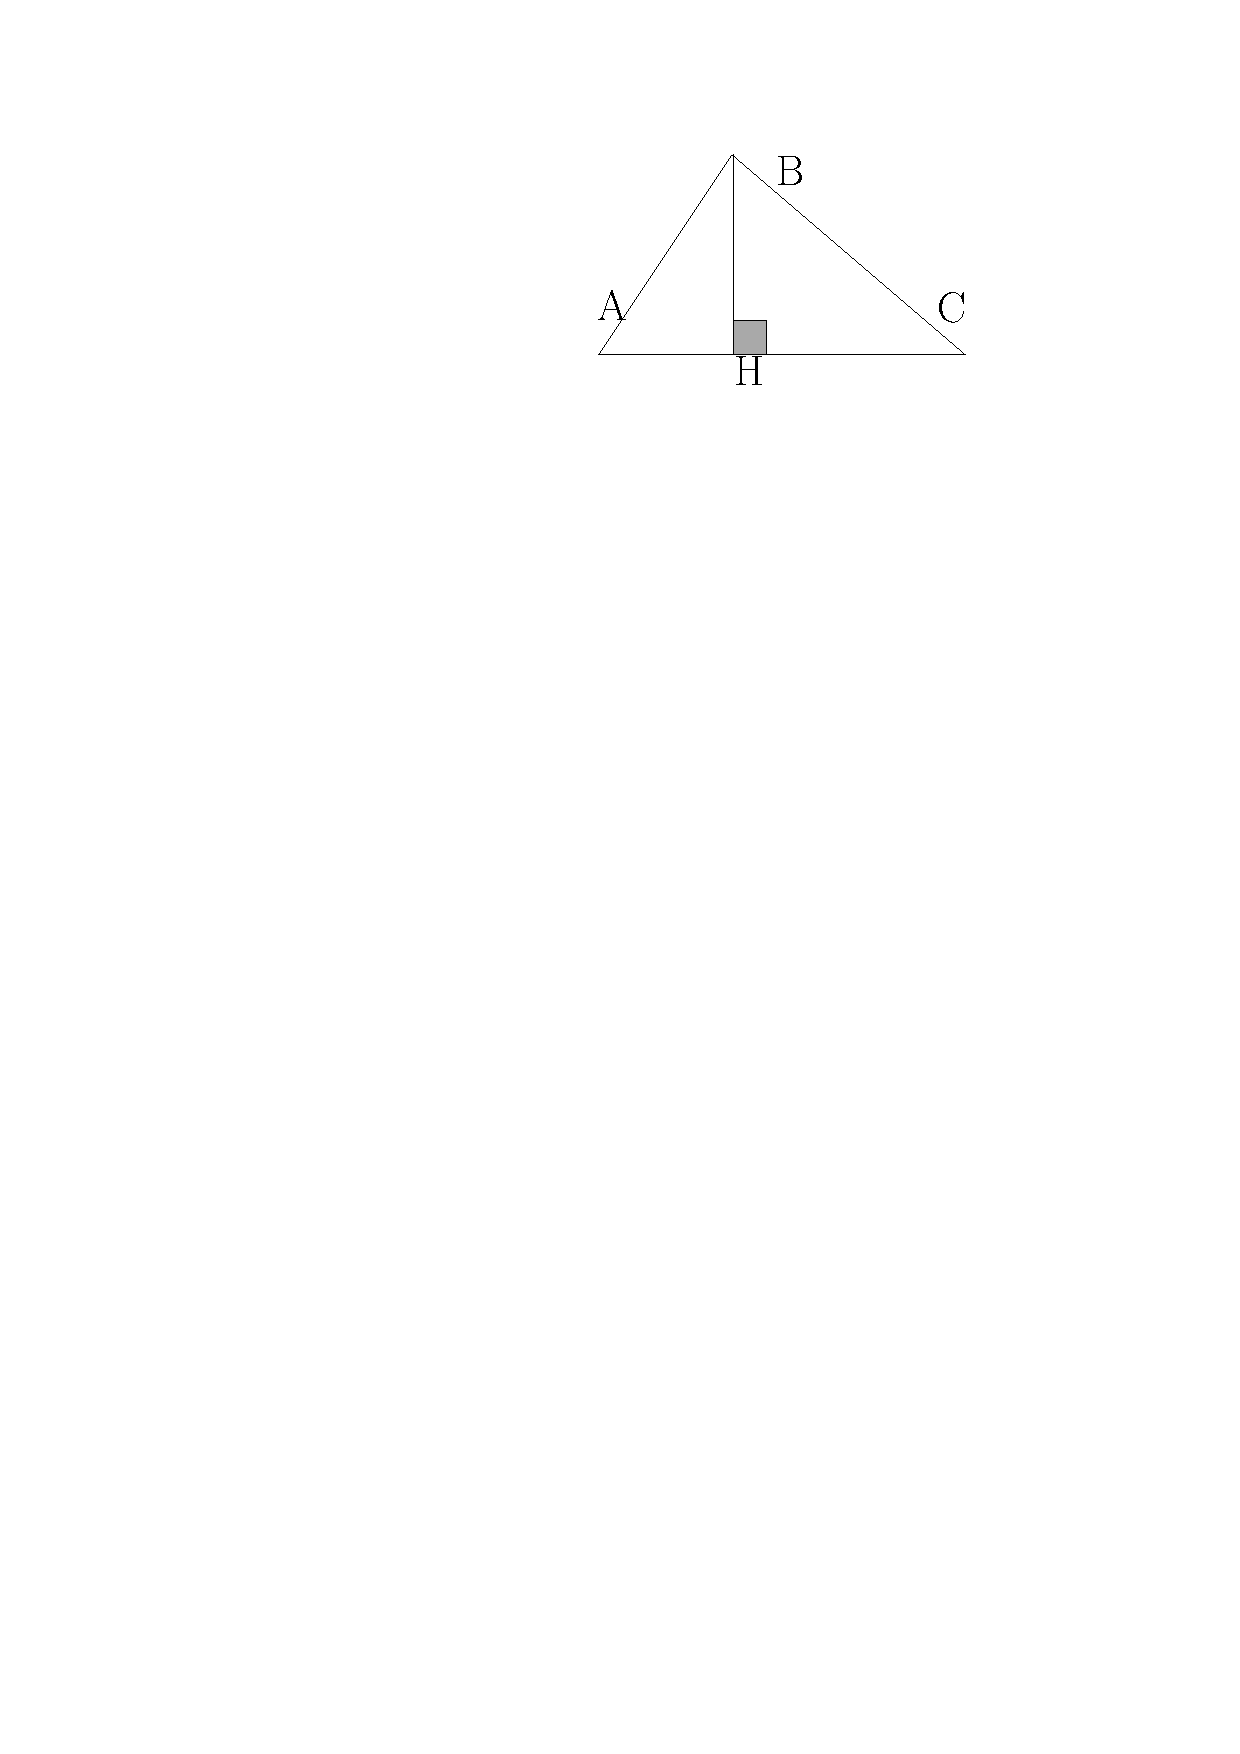
\includegraphics[width=0.8\linewidth]{5x2-geometrie-quadrillage/exo4.pdf}
\end{figure}
\end{minipage}
\subsection*{Exercice 5 - Tracer des droites parallèles}

\textit{Tracer les 3 droites parallèles passant par A, B puis C.}

\begin{figure}[H]
  \centering
  \includegraphics[width=0.6\linewidth]{5x2-geometrie-quadrillage/exo5.pdf}
\end{figure}

\subsection*{Pixel Art}


\begin{multicols}{2}
\begin{figure}[H]
  \centering
  \includegraphics[width=0.8\linewidth]{5x2-geometrie-quadrillage/pixel-art-1.pdf}
\end{figure}

\begin{figure}[H]
  \centering
  \includegraphics[width=0.8\linewidth]{5x2-geometrie-quadrillage/pixel-art-0.pdf}
\end{figure}
\end{multicols}

\subsection*{Graphique}


\begin{multicols}{2}
\begin{figure}[H]
  \centering
  \includegraphics[width=0.8\linewidth]{5x2-geometrie-quadrillage/pixel-art-2.pdf}
\end{figure}

\begin{figure}[H]
  \centering
  \includegraphics[width=0.8\linewidth]{5x2-geometrie-quadrillage/pixel-art-0.pdf}
\end{figure}
\end{multicols}
\end{document}